% Intended LaTeX compiler: pdflatex
\documentclass[10pt,a4paper,UTF8]{article}
\usepackage{zclorg}
\usepackage{tikztheorem}
\author{张朝龙}
\date{}
\title{泊松分布}
\hypersetup{
 pdfauthor={张朝龙},
 pdftitle={泊松分布},
 pdfkeywords={probability},
 pdfsubject={},
 pdfcreator={Emacs 25.0.50.1 (Org mode 9.0.6)},
 pdflang={English}}
\begin{document}

\maketitle
\tableofcontents
\titlepic{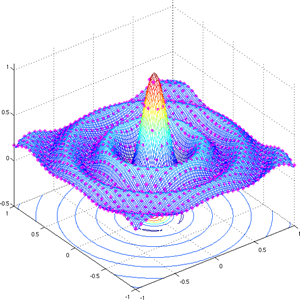
\includegraphics[scale=0.25]{../../img/sinc.PNG}}

\section{定义}
\label{sec:org60bf5b3}


在 \href{binary-distribution.org}{二项分布} 一文中,我们介绍了二项分布的定义和性质。在本文中,我们给出泊松分布,并分析泊松分布和二项分布之间的联系。

\begin{definition}
如果一个取值于\(0,1,2,\ldots\)的随机变量对某一个\(\lambda\),其分布如下:
\begin{equation}
\label{eq:1}
p(i) = P\{X=i\} = e^{-\lambda}\frac{\lambda^{i}}{i!}, i = 0,1,2,\ldots
\end{equation}
则称该随机变量未服从参数\(\lambda\)的泊松随机变量。
\end{definition}
显然:
\begin{equation}
\label{eq:2}
\sum_{i=0}^{\infty}p(i) = \sum_{i=0}^{\infty} e^{-\lambda}\frac{\lambda^{i}}{i!} = 1
\end{equation}
\section{泊松分布与二项分布之间的关系}
\label{sec:orgc3c3a14}


泊松分布在各个领域都有广泛应用,这是由于当\(n\)足够大,\(p\)充分小,\(np\)保持适当的大小时,参数为\((n,p)\)的二项随机变量可以近似的看做参数为\(\lambda = np\)的泊松随机变量。

假设\(X\)是一个服从参数为\((n,p)\)的二项随机变量,并记\(\lambda = np\),那么:
\begin{eqnarray}
\label{eq:3}
P\{X=i\}&=& \binom{n}{i} p^{i}(1-p)^{n-i} \\
&=& \frac{ n! }{(n-i)!i!}(\frac{\lambda}{n})^{i}(1-\frac{\lambda}{n})^{n-i} \\
&=& \frac{n(n-1)\ldots (n-i+1)}{n^{i}} \frac{\lambda^{i}}{i!} \frac{ (1-\lambda/n)^{n} }{ (1- \lambda/n)^{i}  }
\end{eqnarray}
当\(n\to \infty\)时,观察上式:
\begin{eqnarray}
\label{eq:4}
e^{-\lambda}&\approx& (1-\lambda/n)^{n} \\
1&\approx& \frac{n(n-1)\ldots (n-i+1)}{n^{i}} \\
1 &\approx& (1-\frac{\lambda}{n})^{i}
\end{eqnarray}
因此有:
\begin{equation}
\label{eq:5}
P\{ X=i\} \approx e^{-\lambda} \frac{\lambda^{i}}{i!}
\end{equation}

独立重复\(n\)次试验,每次成功的概率为\(p\),当\(n\)充分大,而\(p\)足够小,使得\(np\)保持适当的话,那么成功的次数近似的服从参数为\(\lambda =  np\)的泊松分布,这个\(\lambda\)值通常凭经验确定。

以下的例子大都服从泊松分布:
\begin{enumerate}
\item 一本书里一页或若干页中印刷错误的数量;
\item 某地区居民活到100岁的人数;
\item 一天中拨错电话号码的次数;
\item 一家便利店里每天卖出狗粮饼干的盒数;
\item 某一天进入一个邮局的顾客数;
\end{enumerate}

\section{泊松分布的期望和方差}
\label{sec:orgf0a2a5b}

回忆在上一章节中我们假设\(np=\lambda\),而二项分布的期望是\(np\),另外二项分布的方差是\(np(1-p) = \lambda (1-p)\) 当\(p\)很小时,\(\lambda (1-p)\)近似为\(\lambda\)。所以我们猜测泊松分布的均值和方差都是\(\lambda\)。接下来,证明这一点:
\begin{eqnarray}
\label{eq:6}
E[X]&=& \sum_{i=0}^{\infty} \frac{i e^{-\lambda} \lambda^{i}}{i!} \\
&=& \lambda \sum_{i=1}^{\infty} \frac{ e^{-\lambda} \lambda^{i-1} }{ (i-1)!} \\
&=& \lambda
\end{eqnarray}
上面的推导过程中使用了哑元变量替换。接下来推倒泊松分布的方差:
\begin{eqnarray}
\label{eq:7}
E[X^{2}]&=& \sum_{i=0}^{\infty} \frac{i^{2} e^{-\lambda \lambda^{i}}}{i!} \\
&=& e^{-\lambda} \sum_{i=0}^{\infty} \frac{ \lambda^{i}i }{ (i-1)!} \\
&=& e^{-\lambda} \sum_{i=0}^{\infty} \bigg[ \frac{\lambda^{i}(i-1)}{ (i-1)!}  + \frac{\lambda^{i}}{(i-1)!} \bigg] \\
&=& e^{-\lambda}\sum_{i=0}^{\infty} \lambda \frac{\lambda^{i-1}(i-1)}{(i-1)!} + e^{-\lambda}\sum_{i=0}^{\infty} \frac{\lambda^{i-1}\lambda}{(i-1)!} \\
&=& \lambda E[X] + \lambda \\
&=& \lambda^{2} + \lambda
\end{eqnarray}

根据方差公式:
\begin{eqnarray}
\label{eq:8}
\mathrm{Var}(X)&=& E[X^{2}] - (E[x])^{2} = \lambda \\
\end{eqnarray}
\section{计算泊松分布}
\label{sec:org96ce01b}


如果\(X\)服从参数为\(\lambda\)的泊松分布,则:
\begin{eqnarray}
\label{eq:9}
\frac{P\{X=i+1\} }{P\{X=i\}}&=& \frac{ e^{-\lambda} \lambda^{i+1}/ (i+1)! }{ e^{-\lambda} \lambda^{i}/ i! } \\
&=& \frac{\lambda}{i+1}
\end{eqnarray}
因此,我们有递推式:
\begin{equation}
\label{eq:10}
P\{ X = i +1 \} = \frac{\lambda}{i+1} P\{X=i\}
\end{equation}
\section{使用python做试验}
\label{sec:orgbfcdaad}


在scipy提供的众多科学计算程序中, \texttt{stats} 包含了众多对泊松分布的支持。

我们首先验证当二项分布的\(N\)和\(p\)满足一定条件时,可以用泊松分布来近似的这个结论。

假设\((n,p) = (100,0.1)\),另外假设\(\lambda = 10\),我们有:

\lstset{language=Python,label= ,caption= ,captionpos=b,firstnumber=1,numbers=left}
\begin{lstlisting}
from scipy.stats import binom
import numpy as np
import matplotlib.pyplot as plt
from scipy import stats as S
N,p = 100,0.1
mu = 10
x = np.arange(0,N+1,1)
y_binomial = S.binom.pmf(x,N,p)
y_poisson = S.poisson.pmf(x,mu)
fig,ax = plt.subplots()
ax.plot(x,y_binomial,'-bo',
        label='binomial distribution');
ax.plot(x,y_poisson,'-ro',
        label='poisson distribution');

legend = ax.legend(loc='best',
         shadow=True,
         fontsize='x-large')
legend.get_frame().set_facecolor('#00FFCC')
plt.show()

\end{lstlisting}

结果如图\ref{fig:org6bdfa2e} 所示:
\begin{figure}[htbp]
\centering
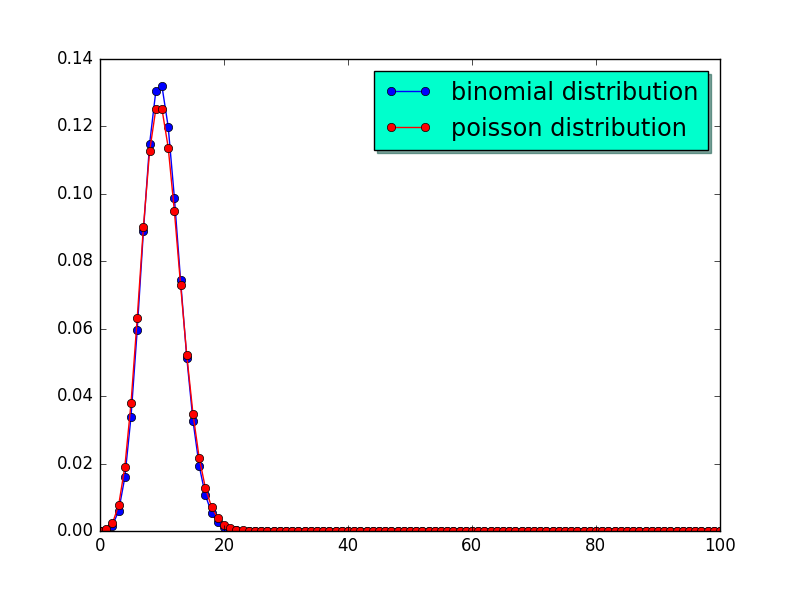
\includegraphics[width=0.6\textwidth]{../../img/math_probability/20170701binomialvspoisson1.png}
\caption{\label{fig:org6bdfa2e}
\((100,0.1)\)的二项分布和\(\lambda = 10\)的泊松分布}
\end{figure}


可以看到当\(np = \lambda\)时,泊松分布和二项分布近似的相当好。事实上当\(n=10,p=0.1,\lambda = np = 1\),或者\(n = 10, p = 0.2,\lambda = np =2\)时,泊松分布和二项分布近似的也相当好。图\ref{fig:org1dbf04c} 直观的展示了这一结论。
\begin{figure}[htbp]
\centering
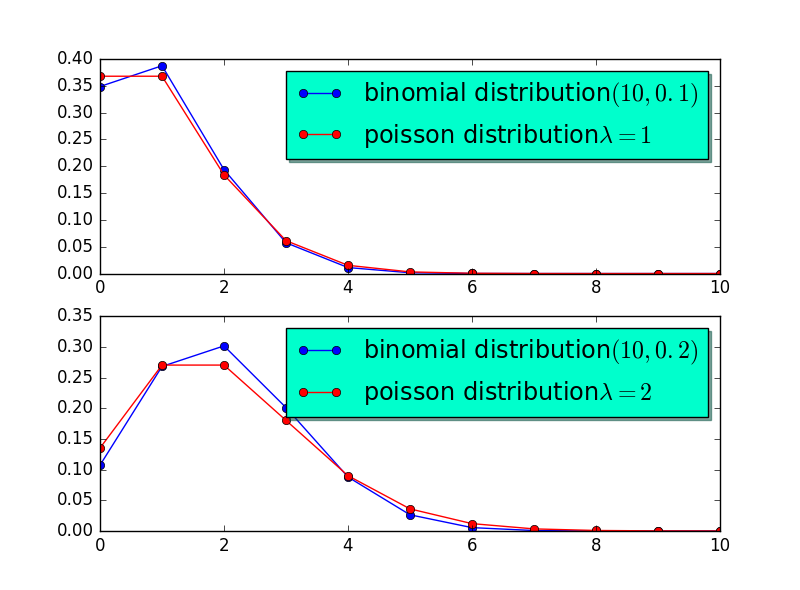
\includegraphics[width=0.6\textwidth]{../../img/math_probability/20170701binomialvspoisson2.png}
\caption{\label{fig:org1dbf04c}
\(np=\lambda\)的二项分布和\(\lambda = 10\)的泊松分布}
\end{figure}

代码如下:

\lstset{language=Python,label= ,caption= ,captionpos=b,firstnumber=1,numbers=left}
\begin{lstlisting}
from scipy.stats import binom
import numpy as np
import matplotlib.pyplot as plt
from scipy import stats as S
N,p = 10,0.1
mu = 1
x = np.arange(0,N+1,1)
y_binomial = S.binom.pmf(x,N,p)
y_poisson = S.poisson.pmf(x,mu)

fig = plt.figure(1)
ax1 = plt.subplot(211)
ax2 = plt.subplot(212)

ax1.plot(x,y_binomial,'-bo',
         label='binomial distribution$(10,0.1)$');
ax1.plot(x,y_poisson,'-ro',
         label='poisson distribution$\lambda = 1$');

legend1 = ax1.legend(loc='best',
                    shadow=True,
                    fontsize='x-large')
legend1.get_frame().set_facecolor('#00FFCC')

N,p = 10,0.2
mu = 2
x = np.arange(0,N+1,1)
y_binomial = S.binom.pmf(x,N,p)
y_poisson = S.poisson.pmf(x,mu)

ax2.plot(x,y_binomial,'-bo',
         label='binomial distribution$(10,0.2)$');
ax2.plot(x,y_poisson,'-ro',
         label='poisson distribution$\lambda=2$');

legend2 = ax2.legend(loc='best',
                    shadow=True,
                    fontsize='x-large')

legend2.get_frame().set_facecolor('#00FFCC')
plt.show()
\end{lstlisting}

现在我们生成10000个\(\lambda=2\)的泊松分布样本。
\lstset{language=Python,label= ,caption= ,captionpos=b,numbers=none}
\begin{lstlisting}
s = S.poisson.rvs(1,size= 1000)
\end{lstlisting}
然后求其均值和方差:
\lstset{language=Python,label= ,caption= ,captionpos=b,numbers=none}
\begin{lstlisting}
np.mean(s)
np.var(s)
\end{lstlisting}
输出为1.04和1.1044。可以预见当我们对更多样本求均值时,会越来越接近于\(1\). 因为泊松分布的均值和方差相等,随着更多样本的加入, \texttt{np.mean(s)} 和 \texttt{np.var(s)} 的值也会越来越靠近。
\end{document}
